%% Outline:
% - Describe CBOW \cite{mikolov_efficient_2013}
% - Describe skip gram \cite{mikolov_distributed_2013}, \cite{mikolov_efficient_2013}
% - Why were these architectures created? (in the text already)
% - What can you do with these word vectors?
% -- Syntactic similarity (e.g. singular::plural, base::comparative::superlative) \cite{mikolov_linguistic_2013}
% -- Semantic similarity / analogy task (
% 	- France is to Paris as Germany is to Berlin \cite{mikolov_distributed_2013}, see 3 Empirical Results
% 	- What is the word that is similar to small in the same sense as biggest is similar to big? \cite{mikolov_efficient_2013}
% 	- clothing is to shirt as dish is to bowl \cite{mikolov_linguistic_2013}
% 	)
% -- Phrase/Idiom detection \cite{mikolov_distributed_2013}
% - Representing relationships in 2d space
% - Calculation of the cosine distance of these vectors \cite{mikolov_linguistic_2013}
% - The word2vec project
% - Word Embeddings
%
\subsubsection{Word2Vec} % (fold)
\label{sub:word_2_vec}

Several architectures for the calculation of word vectors exist (see\,\cite{mikolov_efficient_2013,mikolov_linguistic_2013} for a more detailed elaboration of these architectures). But according to Mikolov et al., none of these \textit{``architectures has been successfully trained on more than a few hundred of millions of words''}\,\cite[p1]{mikolov_efficient_2013}, as they become computationally very expensive with larger data sets (this also applies to the previously mentioned LDA). Therefore, in 2013, Mikolov et al. proposed two optimized neural network architectures for calculating word vectors at a significantly reduced learning time, which allows to train a language model on data sets with billions of words instead: the \emph{continuous bag-of-words model} (CBOW) and the \emph{continuous skip-gram model}\,\cite{mikolov_efficient_2013}.
\textit{``The CBOW architecture predicts the current word based on the context, and the Skip-gram predicts surrounding words given the current word''}\,\cite{mikolov_efficient_2013}\footnote{Consider e.g. the requirements sentence \textit{``As a smart home owner, I want my smart home to\dots''}. Given the the words ['As', 'a', 'smart', 'owner'] a CBOW based model would be trained to predict the word 'home' as missing. On the other hand, given the word 'home', a skip-gram based model would be trained to predict the words which are most likely to surround the word home, so 'smart' and 'owner'.}. Both are shallow neural network architectures consisting of an input layer, a projection layer and an output layer\,\cite{mikolov_efficient_2013,qiang_topic_2016}. Once the language model is trained on any of these architectures, the projection layer holds a dense representation of any word vector, also called \textit{word embedding}\,\cite{tensorflow_word_embeddings}. Following this method, Mikolov et al. could not only improve the speed of the learning, but they also found the word embeddings calculated using this method to preserve the syntactic and semantic regularities of the input words given to the neural network\,\cite{mikolov_linguistic_2013}. When representing the words in vector space it is then possible, to express these syntactic and semantic similarities by vector offsets, where all pairs of words sharing a particular relation are related by the same constant offset\,\cite{mikolov_linguistic_2013}. \autoref{fig:word_emb_relationships} visualizes these offset-relations in the three-dimensional space. E.g. the \text{Country-Capital} plot shows how the word vectors for countries share similar offsets to the word vectors of the belonging capital. This allows to discover relations between words through algebraic operations with their vector representations. E.g. the analogy \textit{Spain is to Madrid as Germany is to Berlin}, could be mathematically solved by finding the word whose vector is closest to $X = vector("Spain") - vector("Madrid") + vector("Germany")$ measured by cosine distance\,\cite{mikolov_efficient_2013}. In addition to their initial research, Mikolov et al. created the word2vec open-source project, which incorporates the tool they used to create word embeddings from text corpora based on their promoted neural network architectures CBOW and skip-gram\footnote{\label{word2vec_link}\url{https://code.google.com/archive/p/word2vec/}}.

\begin{figure}[ht]
  \centering
    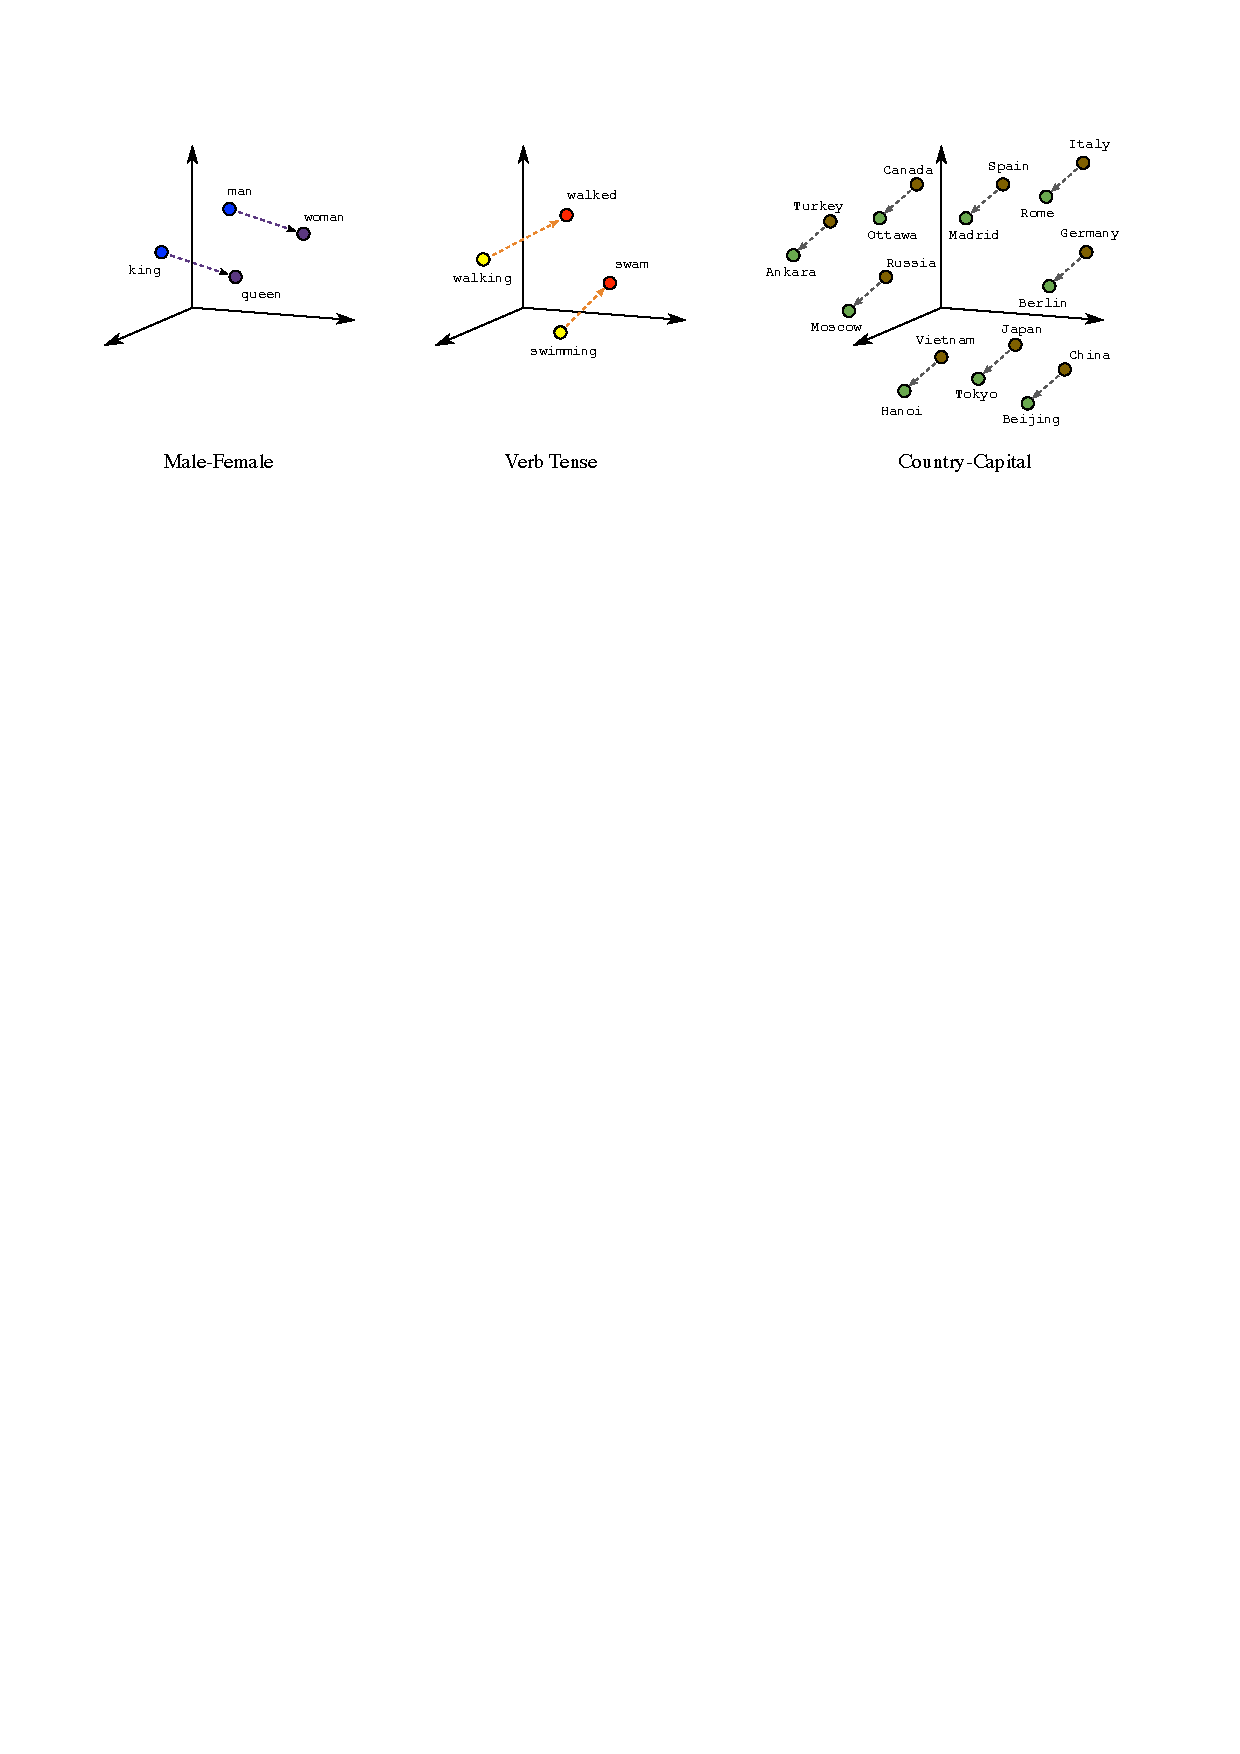
\includegraphics[width=\textwidth]{figures/word-embedding-relationships.pdf}
    \caption{Word analogies visualized using word embeddings in three-dimensional space \,\cite{google_embeddings_figure}.}
    \label{fig:word_emb_relationships}
\end{figure}
\FloatBarrier

\blockcomment{
The   structure   of   CBOW   is   similar   to   a   feed-forward   neural   network, with the exception that the non-linear hidden layer in the   former   is   removed.   By   getting   around   the   heavy   computational burden incurred by the non-linear hidden layer, the  model  can  be  trained  on  a  large  corpus  efficiently,  while  still  retains  good  performance. 
(Paper: Exploring Word Mover’s Distance and Semantic-Aware Embedding Techniques for Extractive Broadcast News Summarization)


Furthermore, the quality of the learned vectors by previous architectures is inherently limited for their "indifference to word order and their inability to represent idiomatic phrases"\cite[p1]{mikolov_distributed_2013}. This limitation was also important for us to consider during our analysis.\\

As a consequence of the user story format imposed to our requirement sentences a larger number of the requirements contained the phrase "I want my smart home to..." ($416 / 2966 \approx14.03\%$). Also, the requested role description induced some of the participants to start their requirements with "As a smart home owner..." (8 requirements). Even though the latter example may be less relevant in its impact on our findings, it illustrates the problem of idioms just perfectly. Because when calculating the word vectors for these phrases using an LDA, the words "smart", "home" and "owner" would be represented by the same vectors. Hence, the phrase "a smart home owner" would always be represented with the same vectors and the vector distance of this phrase would be similar to both of the phrases "a clever home owner" and "an owner of a smart home". Especially after the stop-words were removed. It is rather obvious though, how these phrases could change the meaning of a statement completely.\\
A combination of two words which appear often together is called a bi-gram (or a 2-gram), but more words than just 2 could be involved making it a combination of an arbitrary number of N words and thus an n-gram. To detect these n-grams usually is done using statistical probability models, where one would analyze a given corpus of words to understand what words frequently occur close to each another\cite{suen_n-gram_1979}. The task of finding n-grams also is not just limited to finding related words, but started as a task of finding related characters which would follow one another\cite{cavnar_n-gram-based_nodate} and was a measurement to improve the performance of automatic character recognition systems\cite{suen_n-gram_1979}.\\
In their word2vec library, Mikolov et al. focused on the application for phrase detection though, to maximize the accuracy on the phrase analogy task. Using a dataset with about 33 billion words, they were able to train a model that reached an accuracy of 72\% for the detection of phrase analogies\cite[p6]{mikolov_distributed_2013}.

As discussed earlier, many phrases have a meaning that is not a simple composition of the meanings of its individual words. To learn vector representation for phrases, we first find words that appear frequently together, and infrequently in other contexts. For example, “New York Times” and “Toronto Maple Leafs” are replaced by unique tokens in the training data, while a bi-gram “this is” will remain unchanged.
\cite[p5]{mikolov_distributed_2013} 
}